%! Mode:: "TeX:UTF-8"
%! TEX program = xelatex
\PassOptionsToPackage{quiet}{xeCJK}
\documentclass[withoutpreface,bwprint]{cumcmthesis}
\usepackage{etoolbox}
\BeforeBeginEnvironment{tabular}{\zihao{-5}}
\usepackage[numbers,sort&compress]{natbib}  % 文献管理宏包
\usepackage[framemethod=TikZ]{mdframed}  % 框架宏包
\usepackage{url}  % 网页链接宏包
\usepackage{subcaption}  % 子图宏包
\newcolumntype{C}{>{\centering\arraybackslash}X}
\newcolumntype{R}{>{\raggedleft\arraybackslash}X}
\newcolumntype{L}{>{\raggedright\arraybackslash}X}


\usepackage{multirow}
\usepackage{array}







\title{C题:母亲身心健康对婴儿成长的影响}  % 论文标题
\tihao{}  % 题号
\baominghao{}  % 报名号
\schoolname{}  % 学校
\membera{}  % 队员a
\memberb{}  % 队员b
\memberc{}  % 队员c
\supervisor{}  % 指导老师
\yearinput{}
\monthinput{}
\dayinput{}

%%%%%%%%%%%%%%%%%%%%%%%%%%%%%%%%%%%%%%%%%%%%%%%%%%%%%%%%%%%%%
%% 正文
\begin{document}
\begin{samepage}
\begin{center}
\renewcommand{\arraystretch}{2}
\begin{tabular}{|>{\centering\arraybackslash}m{0.13\textwidth}
                |>{\centering\arraybackslash}m{0.65\textwidth}
                |>{\centering\arraybackslash}m{0.17\textwidth}|}
    \hline
    \songti 所属类别
    & \multirow{2}{*}{\centering\songti\zihao{4} \textbf{2024年“华数杯”全国大学生数学建模竞赛}}
    & \songti 参赛编号 \\
    \cline{1-1} \cline{3-3}
    \songti 本科组 & & CM2400947 \\
    \hline
\end{tabular}
\end{center}

\maketitle

\begin{abstract}


\keywords{keywords1, keywords2, keywords3}
\end{abstract}
\end{samepage}
%%%%%%%%%%%%%%%%%%%%%%%%%%%%%%%%%%%%%%%%%%%%%%%%%%%%%%%%%%%%% 

% \tableofcontents  % 目录
% \newpage

%%%%%%%%%%%%%%%%%%%%%%%%%%%%%%%%%%%%%%%%%%%%%%%%%%%%%%%%%%%%%  
\section{问题重述}
\subsection{问题背景}


%%%%%%%%%%%%%%%%%%%%%%%%%%%%%%%%%%%%%%%%%%%%%%%%%%%%%%%%%%%%% 

\subsection{问题提出}

在以上的问题背景下,结合附件数据集,建立数学模型解决以下问题:

\textbf{问题1}

\textbf{问题2}

%%%%%%%%%%%%%%%%%%%%%%%%%%%%%%%%%%%%%%%%%%%%%%%%%%%%%%%%%%%%% 

\section{问题分析}
\subsection{问题1分析}

\subsection{问题2分析}	

% \begin{figure}[H]
%     \centering
%     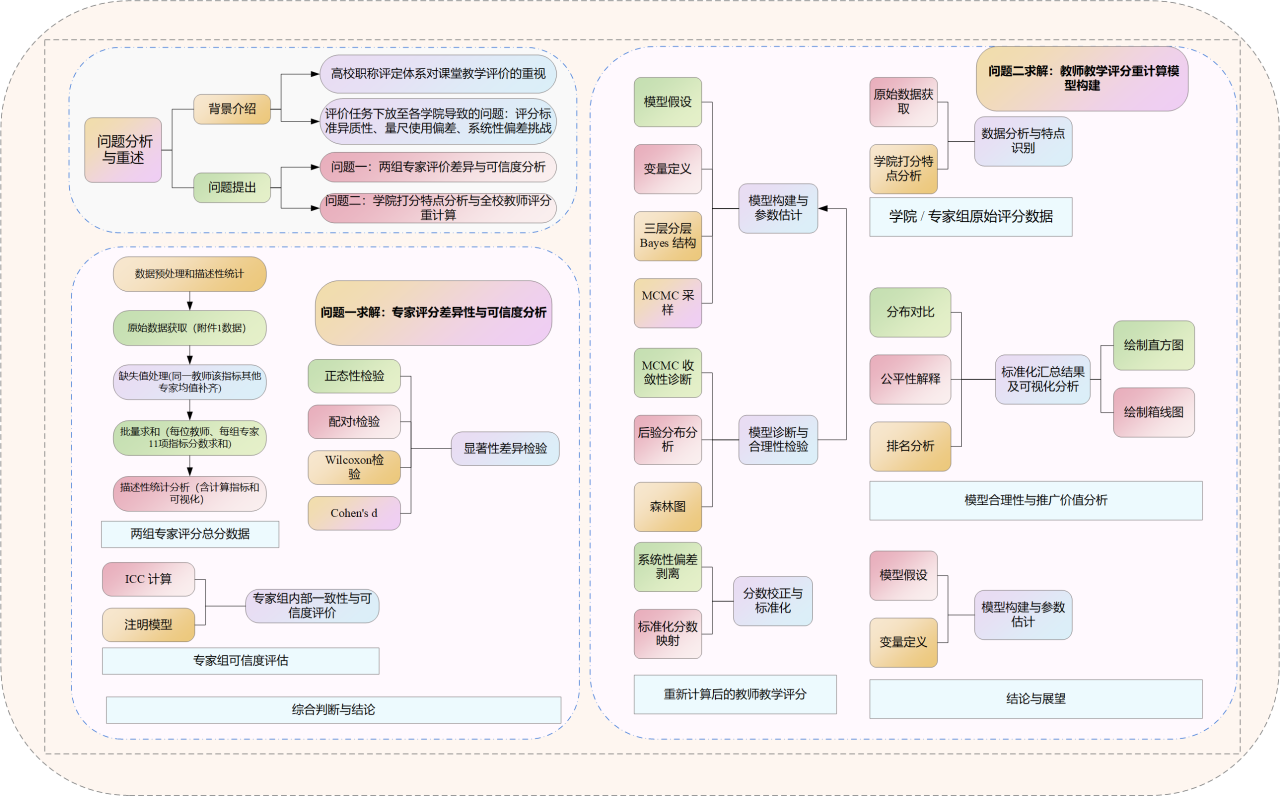
\includegraphics[width=1\textwidth]{figures/flow_chat.png} % 插入图片
%     \caption{方案流程图}
% \end{figure}

%%%%%%%%%%%%%%%%%%%%%%%%%%%%%%%%%%%%%%%%%%%%%%%%%%%%%%%%%%%%% 

\section{模型假设}

为简化问题,本文做出以下假设:

\begin{itemize}
    \item 假设1
    \item 假设2
    \item 假设3
\end{itemize}
%%%%%%%%%%%%%%%%%%%%%%%%%%%%%%%%%%%%%%%%%%%%%%%%%%%%%%%%%%%%% 

% \section{符号说明}
% \begin{table}[H]
% \centering
% \begin{tabularx}{\textwidth}{CLC}
% \toprule
% 符号    & 说明    & 单位 \\
% \midrule
% $m     $& 质量 & $kg$ \\
% $V     $& 体积 & $m^3$ \\

% $S^{(1)}_i$& 第$i$位教师第一组专家的平均总分& 分 \\
% $S^{(2)}_i$& 第$i$位教师第二组专家的平均总分& 分 \\
% $D_i = S^{(1)}_i - S^{(2)}_i$& 第$i$位教师两组评分平均值差异& 分 \\
% $S_{ijk}$& 第$i$学院,第$j$专家组,第$k$教师的原始总分& 分 \\
% $\mu_\text{global}$& 全校教师评分总体均值& 分 \\
% $\alpha_i$& 第$i$学院系统性偏差& 分 \\
% $\beta_{ij}$& 第$i$学院第$j$专家组系统性偏差& 分 \\
% $\epsilon_{ijk}$& 随机扰动,$\epsilon_{ijk} \sim\mathcal{N}(0, \sigma_{error}^2)$& 分 \\
% \bottomrule
% \end{tabularx}
% \label{tab:符号说明}
% \end{table}

\section{符号说明}
\begin{table}[H]
\centering
% \caption{符号说明表}
\begin{tabularx}{\textwidth}{>{\raggedright\arraybackslash}m{3cm} >{\centering\arraybackslash}X >{\centering\arraybackslash}m{2cm}}
\toprule
\textbf{符号}    & \textbf{说明}    & \textbf{单位} \\
\midrule
% $m$                            & 质量                                      & kg \\
% $V$                            & 体积                                      & m$^3$ \\
$S^{(1)}_i$                    & 第 $i$ 位教师第一组专家的平均总分        & 分 \\
$S^{(2)}_i$                    & 第 $i$ 位教师第二组专家的平均总分        & 分 \\
$D_i = S^{(1)}_i - S^{(2)}_i$  & 第 $i$ 位教师两组评分平均值差异          & 分 \\
$S_{ijk}$                      & 第 $i$ 学院,第 $j$ 专家组,第 $k$ 教师的原始总分 & 分 \\
$\mu_\text{global}$            & 全校教师评分总体均值                      & 分 \\
$\alpha_i$                     & 第 $i$ 学院系统性偏差                    & 分 \\
$\beta_{ij}$                   & 第 $i$ 学院第 $j$ 专家组系统性偏差       & 分 \\
$\epsilon_{ijk}$               & 随机扰动,$\epsilon_{ijk} \sim \mathcal{N}(0, \sigma_{error}^2)$ & 分 \\
\bottomrule
\end{tabularx}
\label{tab:符号说明}
\end{table}


%%%%%%%%%%%%%%%%%%%%%%%%%%%%%%%%%%%%%%%%%%%%%%%%%%%%%%%%%%%%% 

\section{问题一的模型建立和求解}

\subsection{问题一的模型的建立和求解}
\subsubsection{模型建立}




% \begin{figure}[ht]
% \centering
% 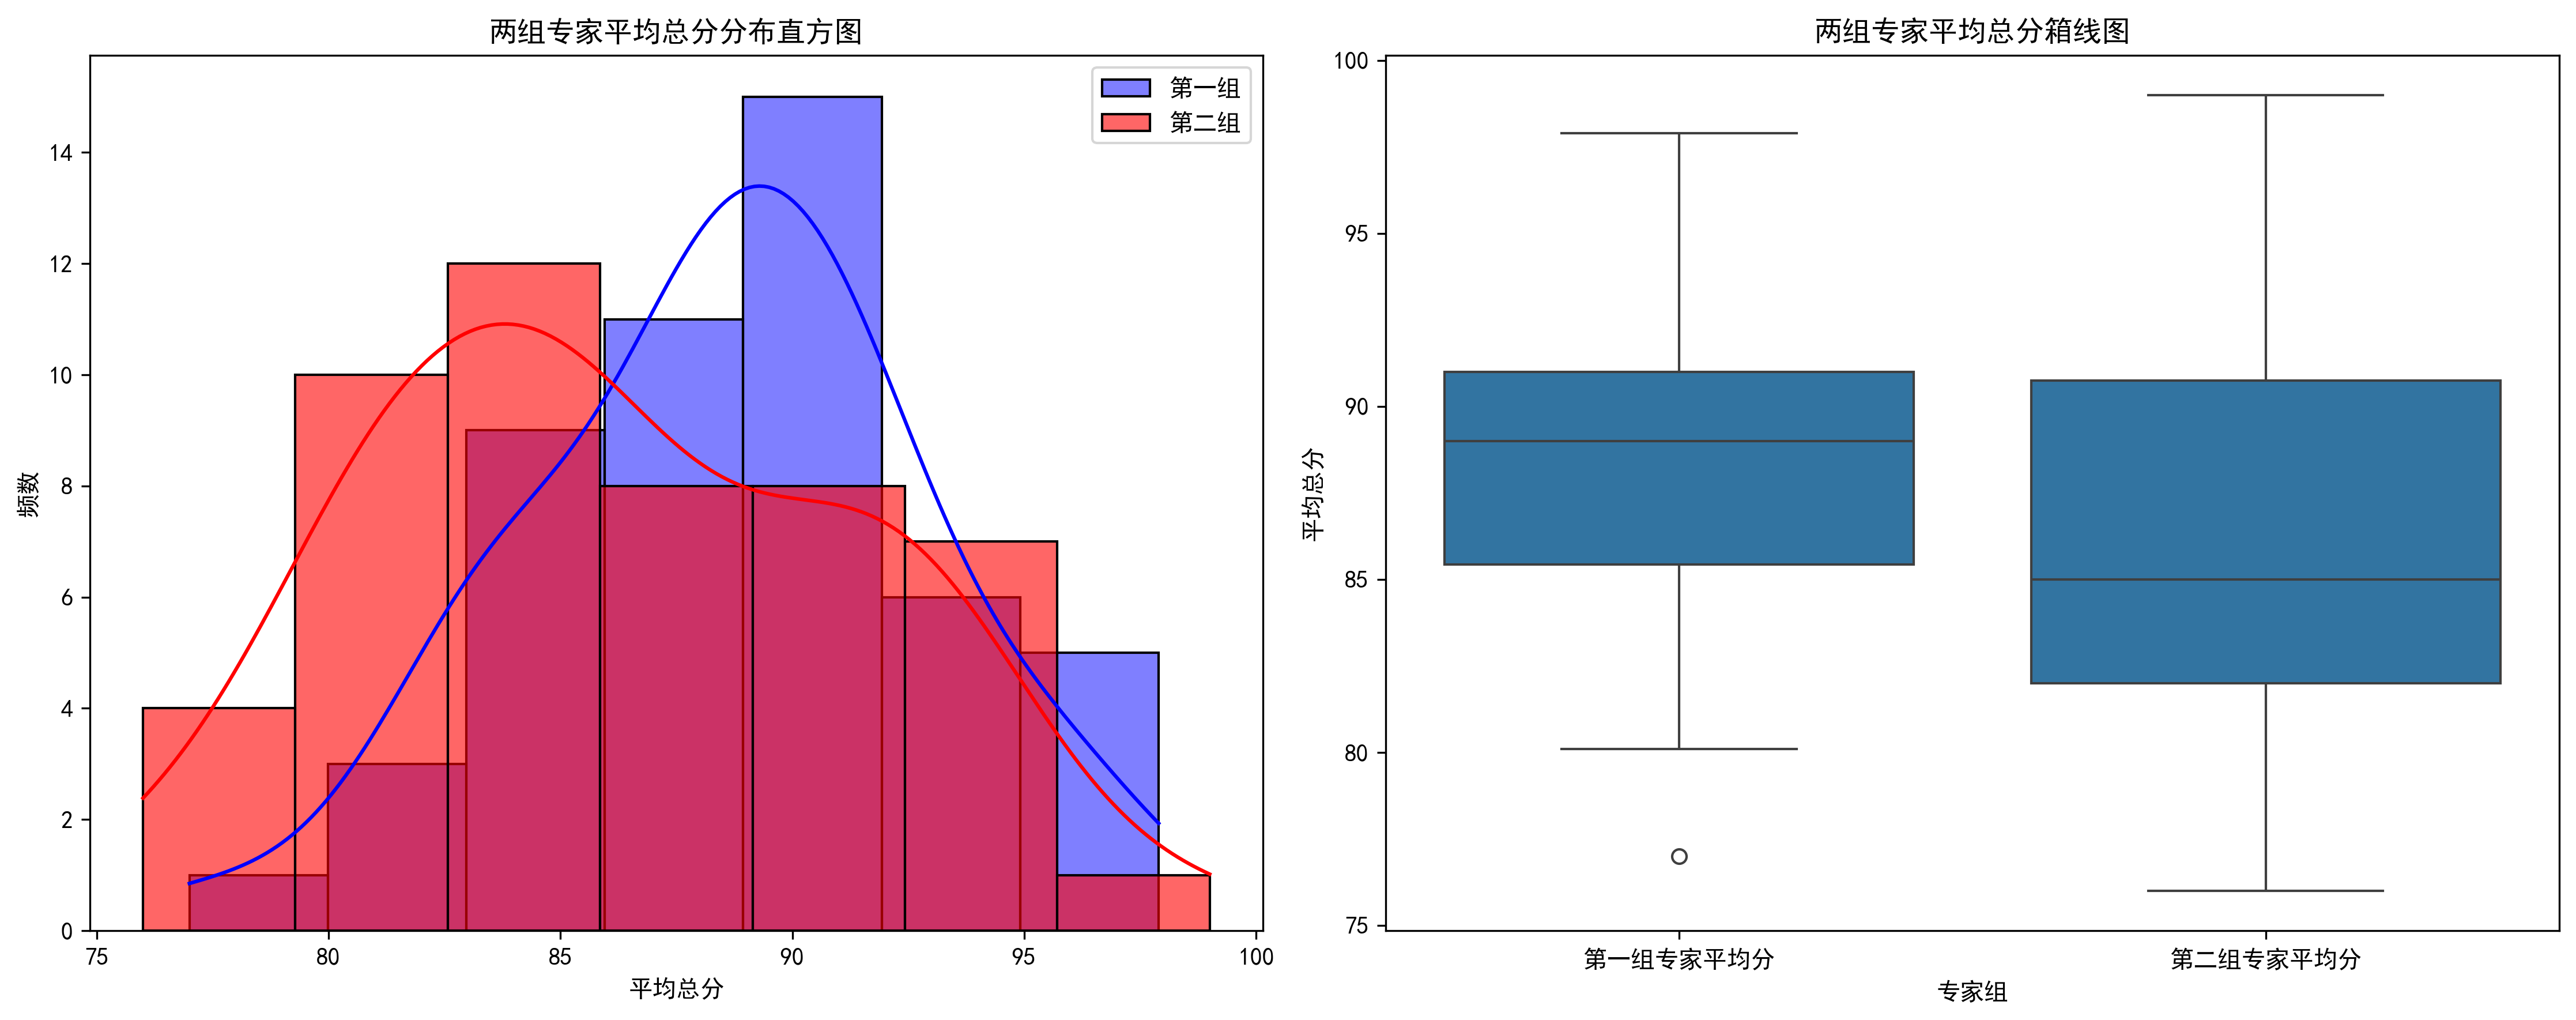
\includegraphics[width=0.75\textwidth]{figures/descriptive_statistics.png}
% % \caption{单图}
% \label{fig:单图}
% \end{figure}

% \begin{figure}[ht]
% \centering
% 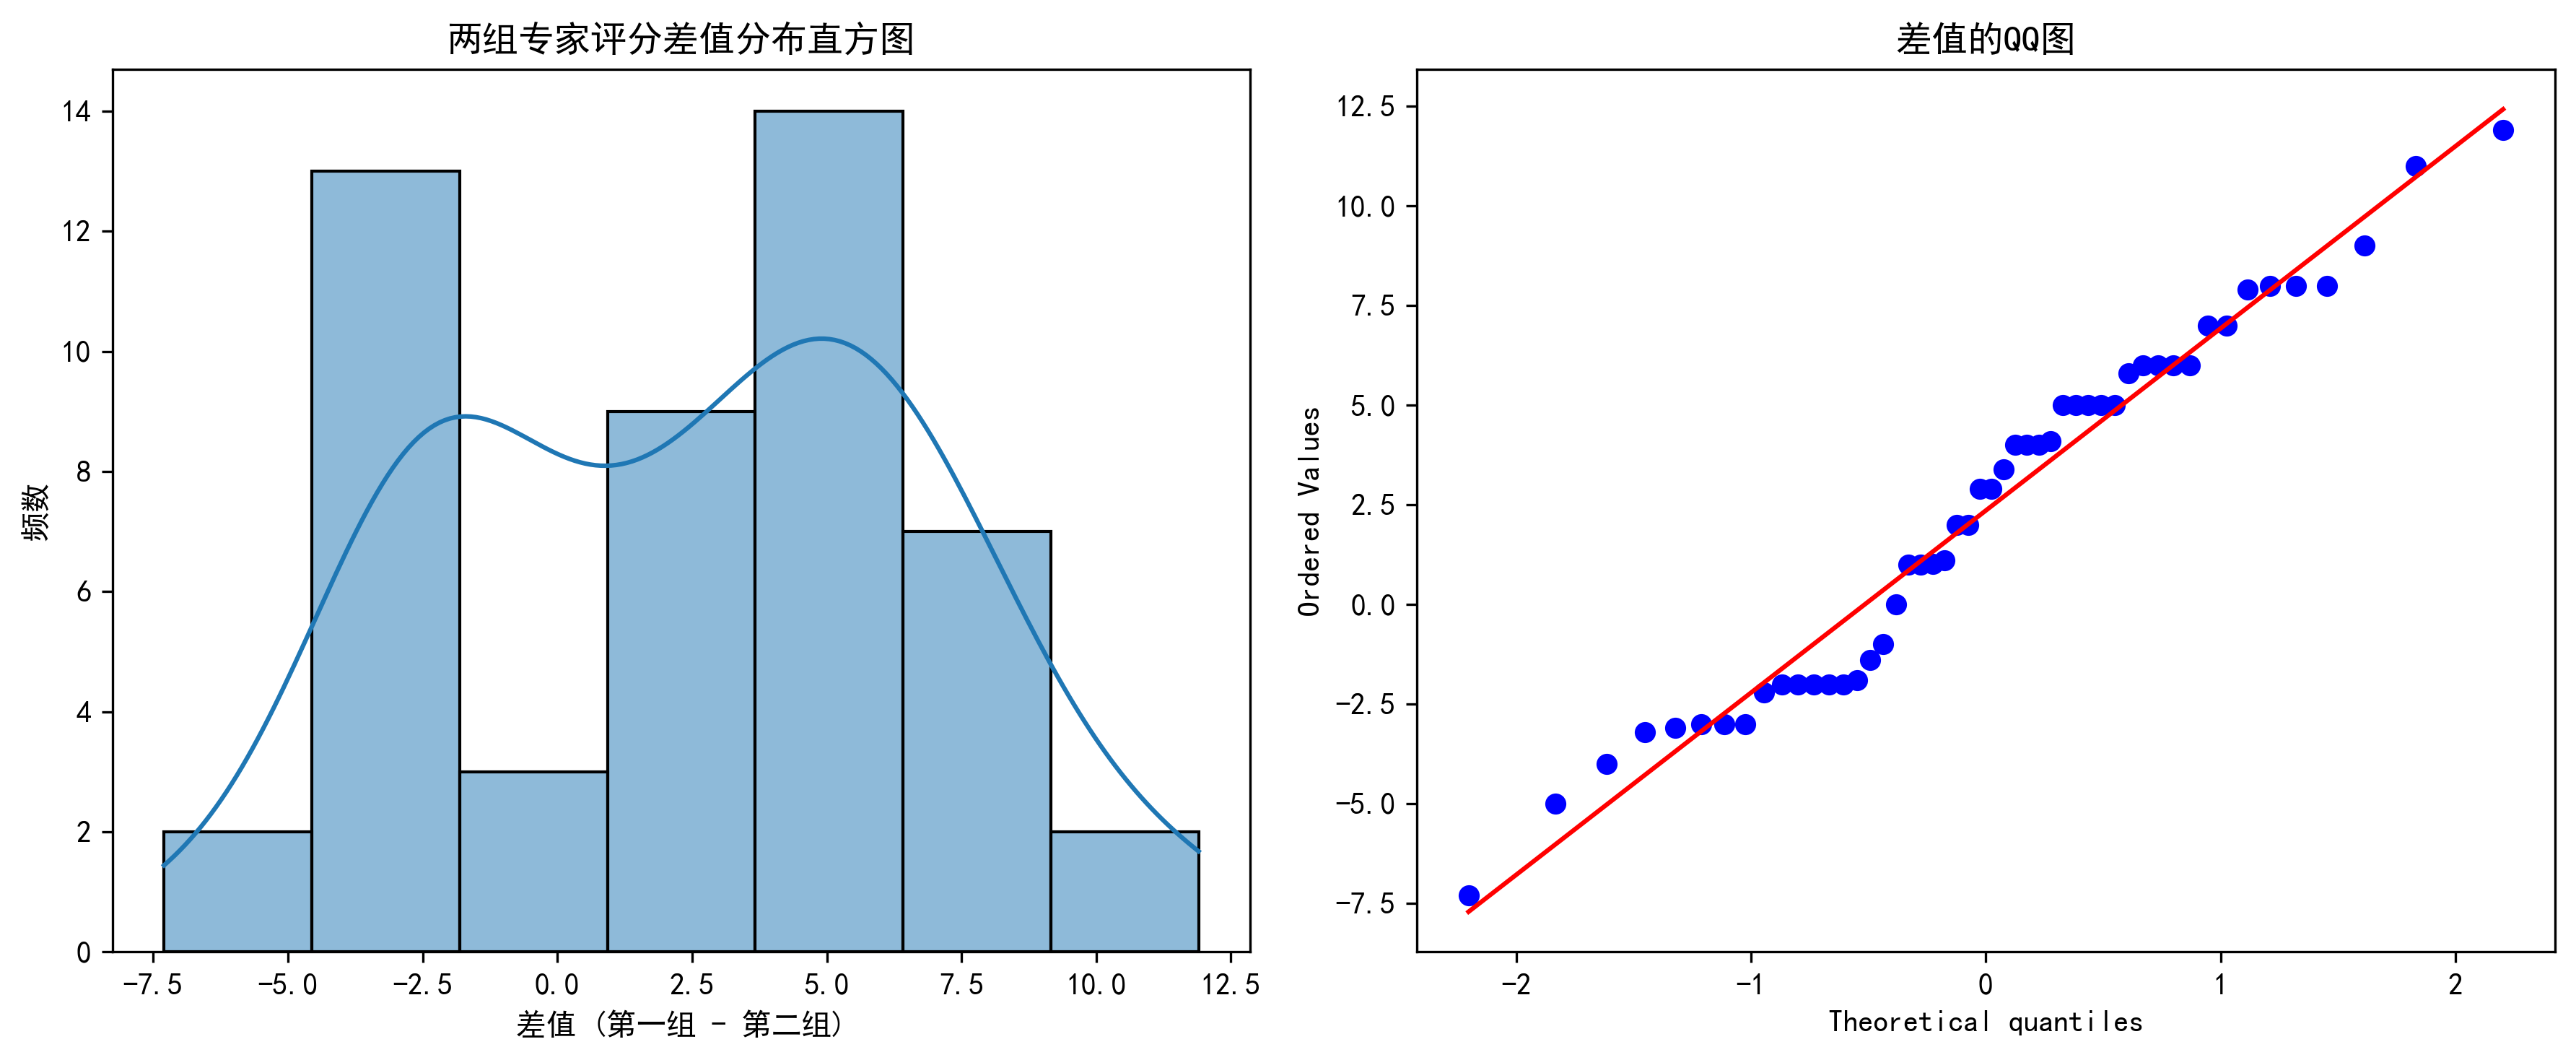
\includegraphics[width=0.75\textwidth]{figures/normality_test.png}
% % \caption{单图}
% \label{fig:单图}
% \end{figure}

% \textbf{Step3:} 组内一致性分析,ICC(2,1)结果分别为:第一组$0.518$(中等一致性),第二组$0.323$(较差)。第一组评分标准和稳定性明显优于第二组。


% \begin{figure}[H]
% \centering
% 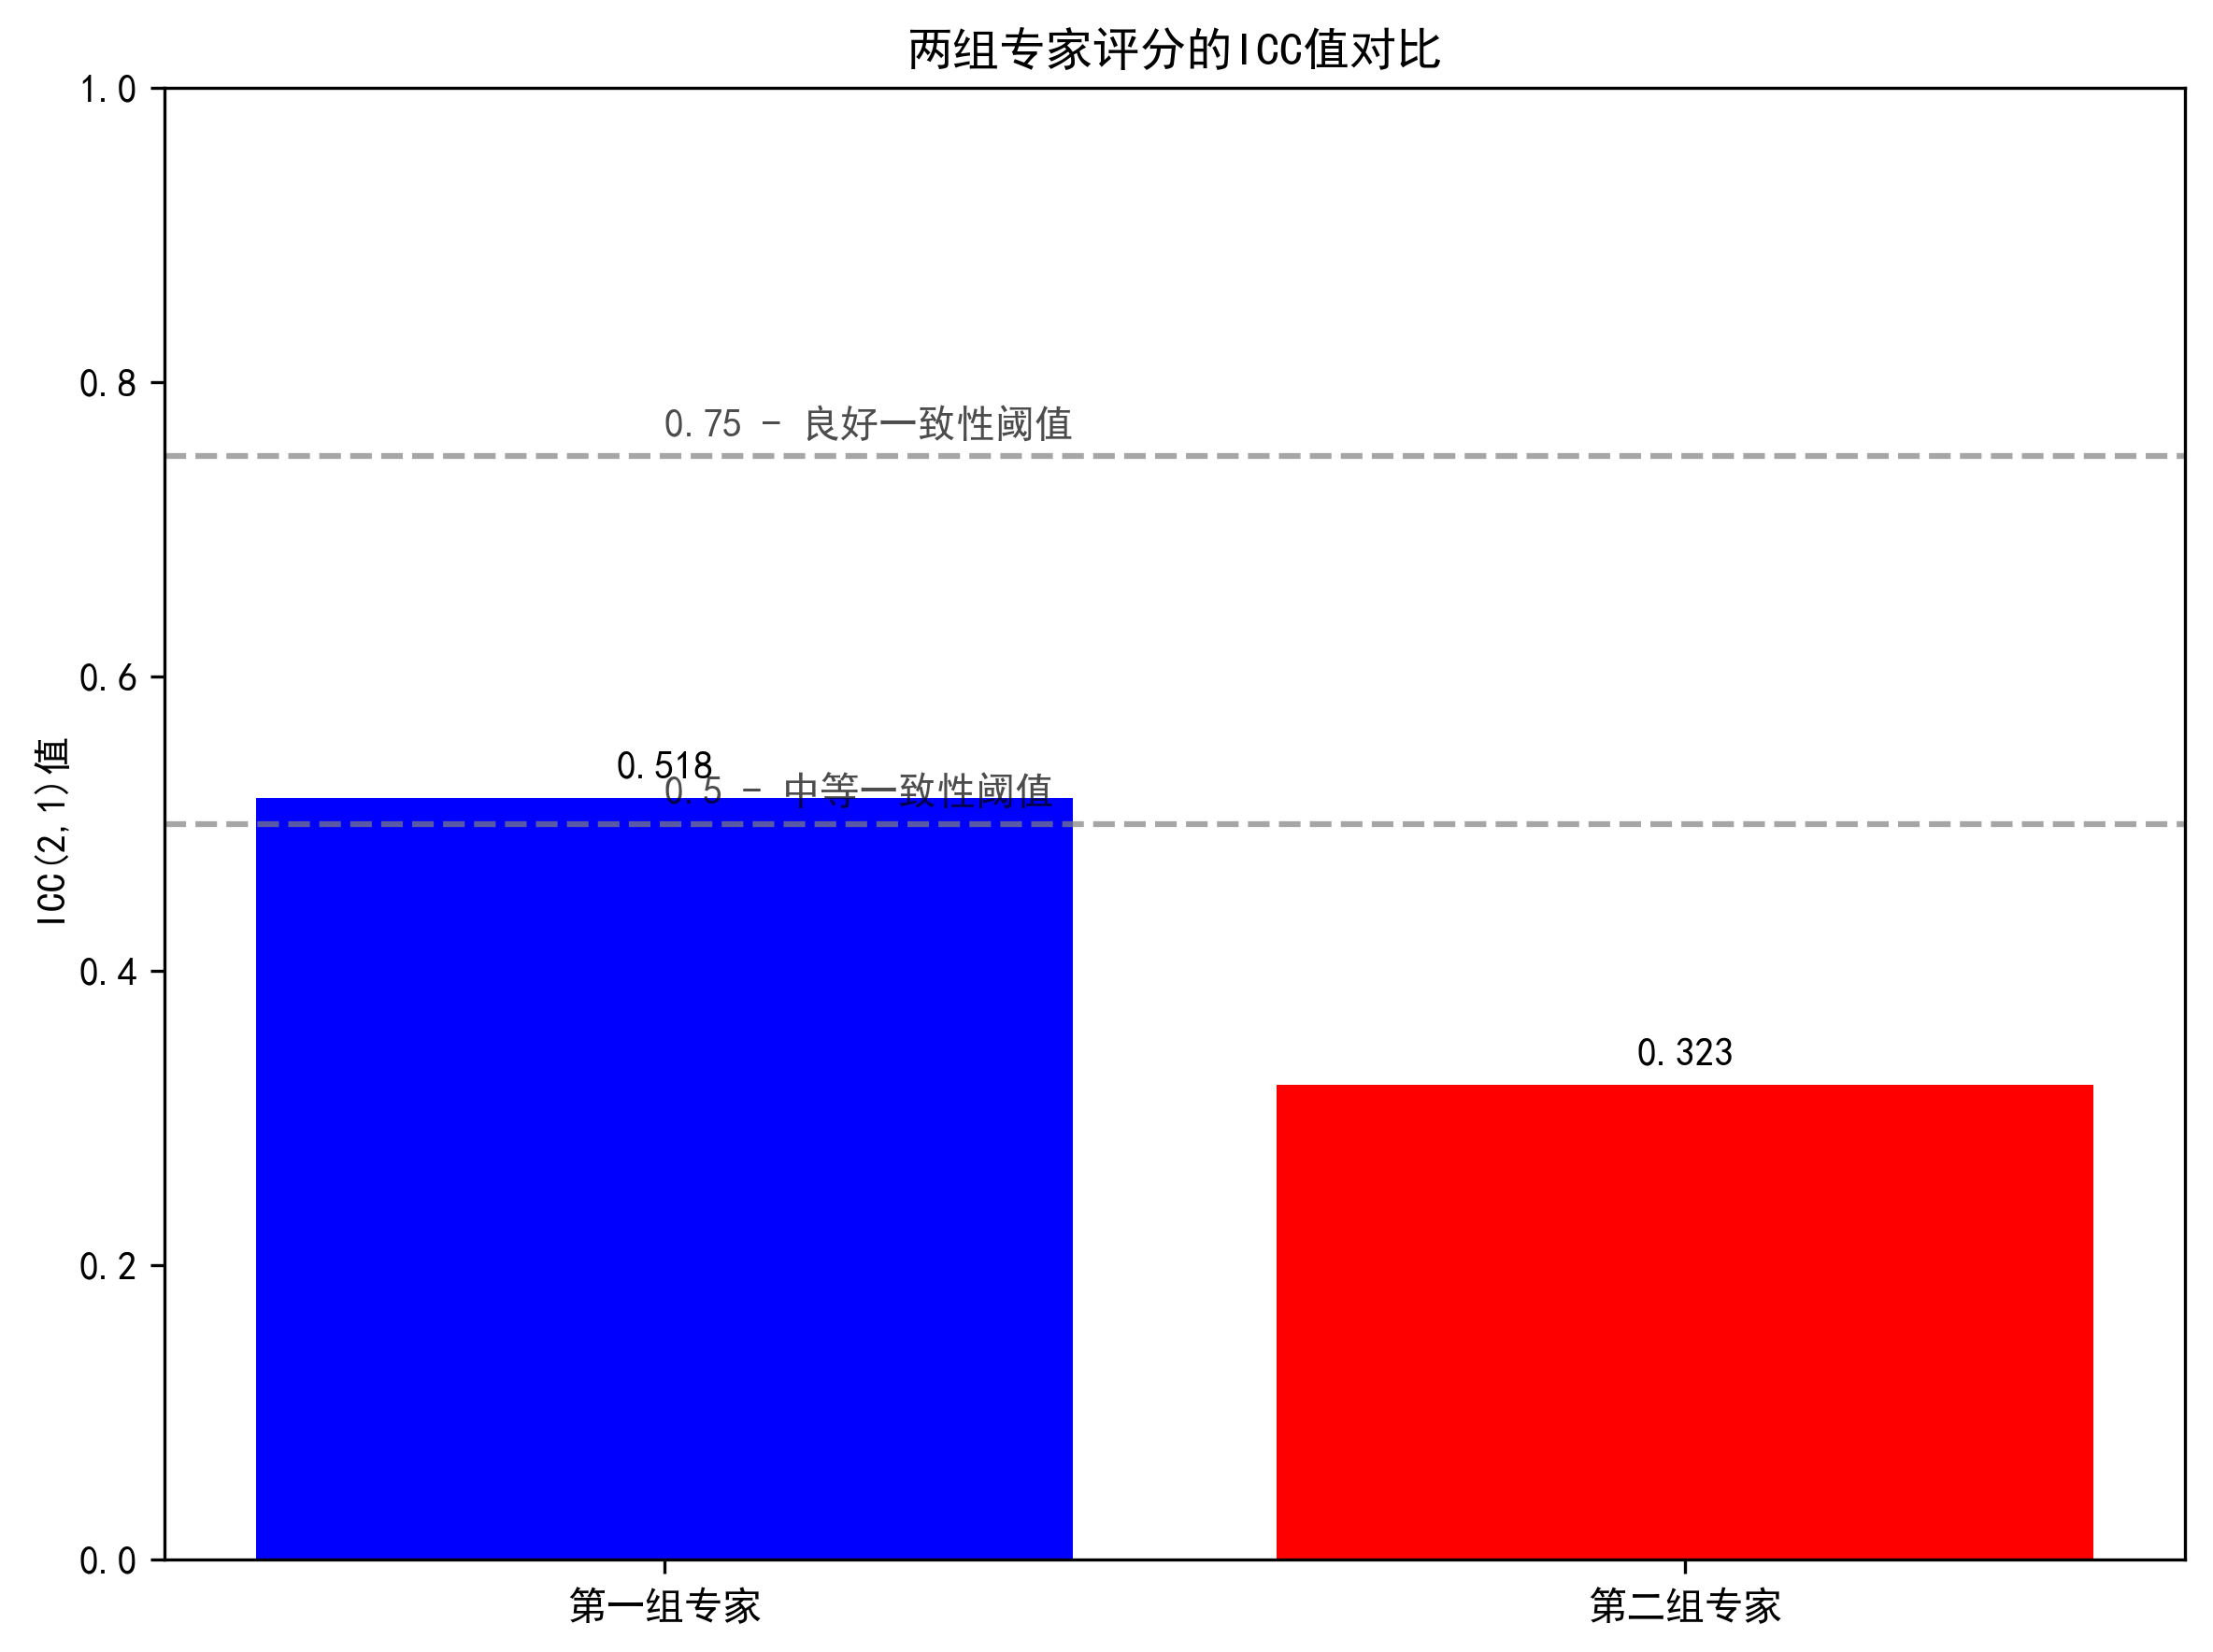
\includegraphics[width=0.75\textwidth]{figures/icc_analysis.png}
% % \caption{单图}
% \label{fig:单图}
% \end{figure}

\subsubsection{求解结果}


\section{问题二的模型建立和求解}
\subsection{模型建立}


% \begin{figure}[H]
% \centering
% 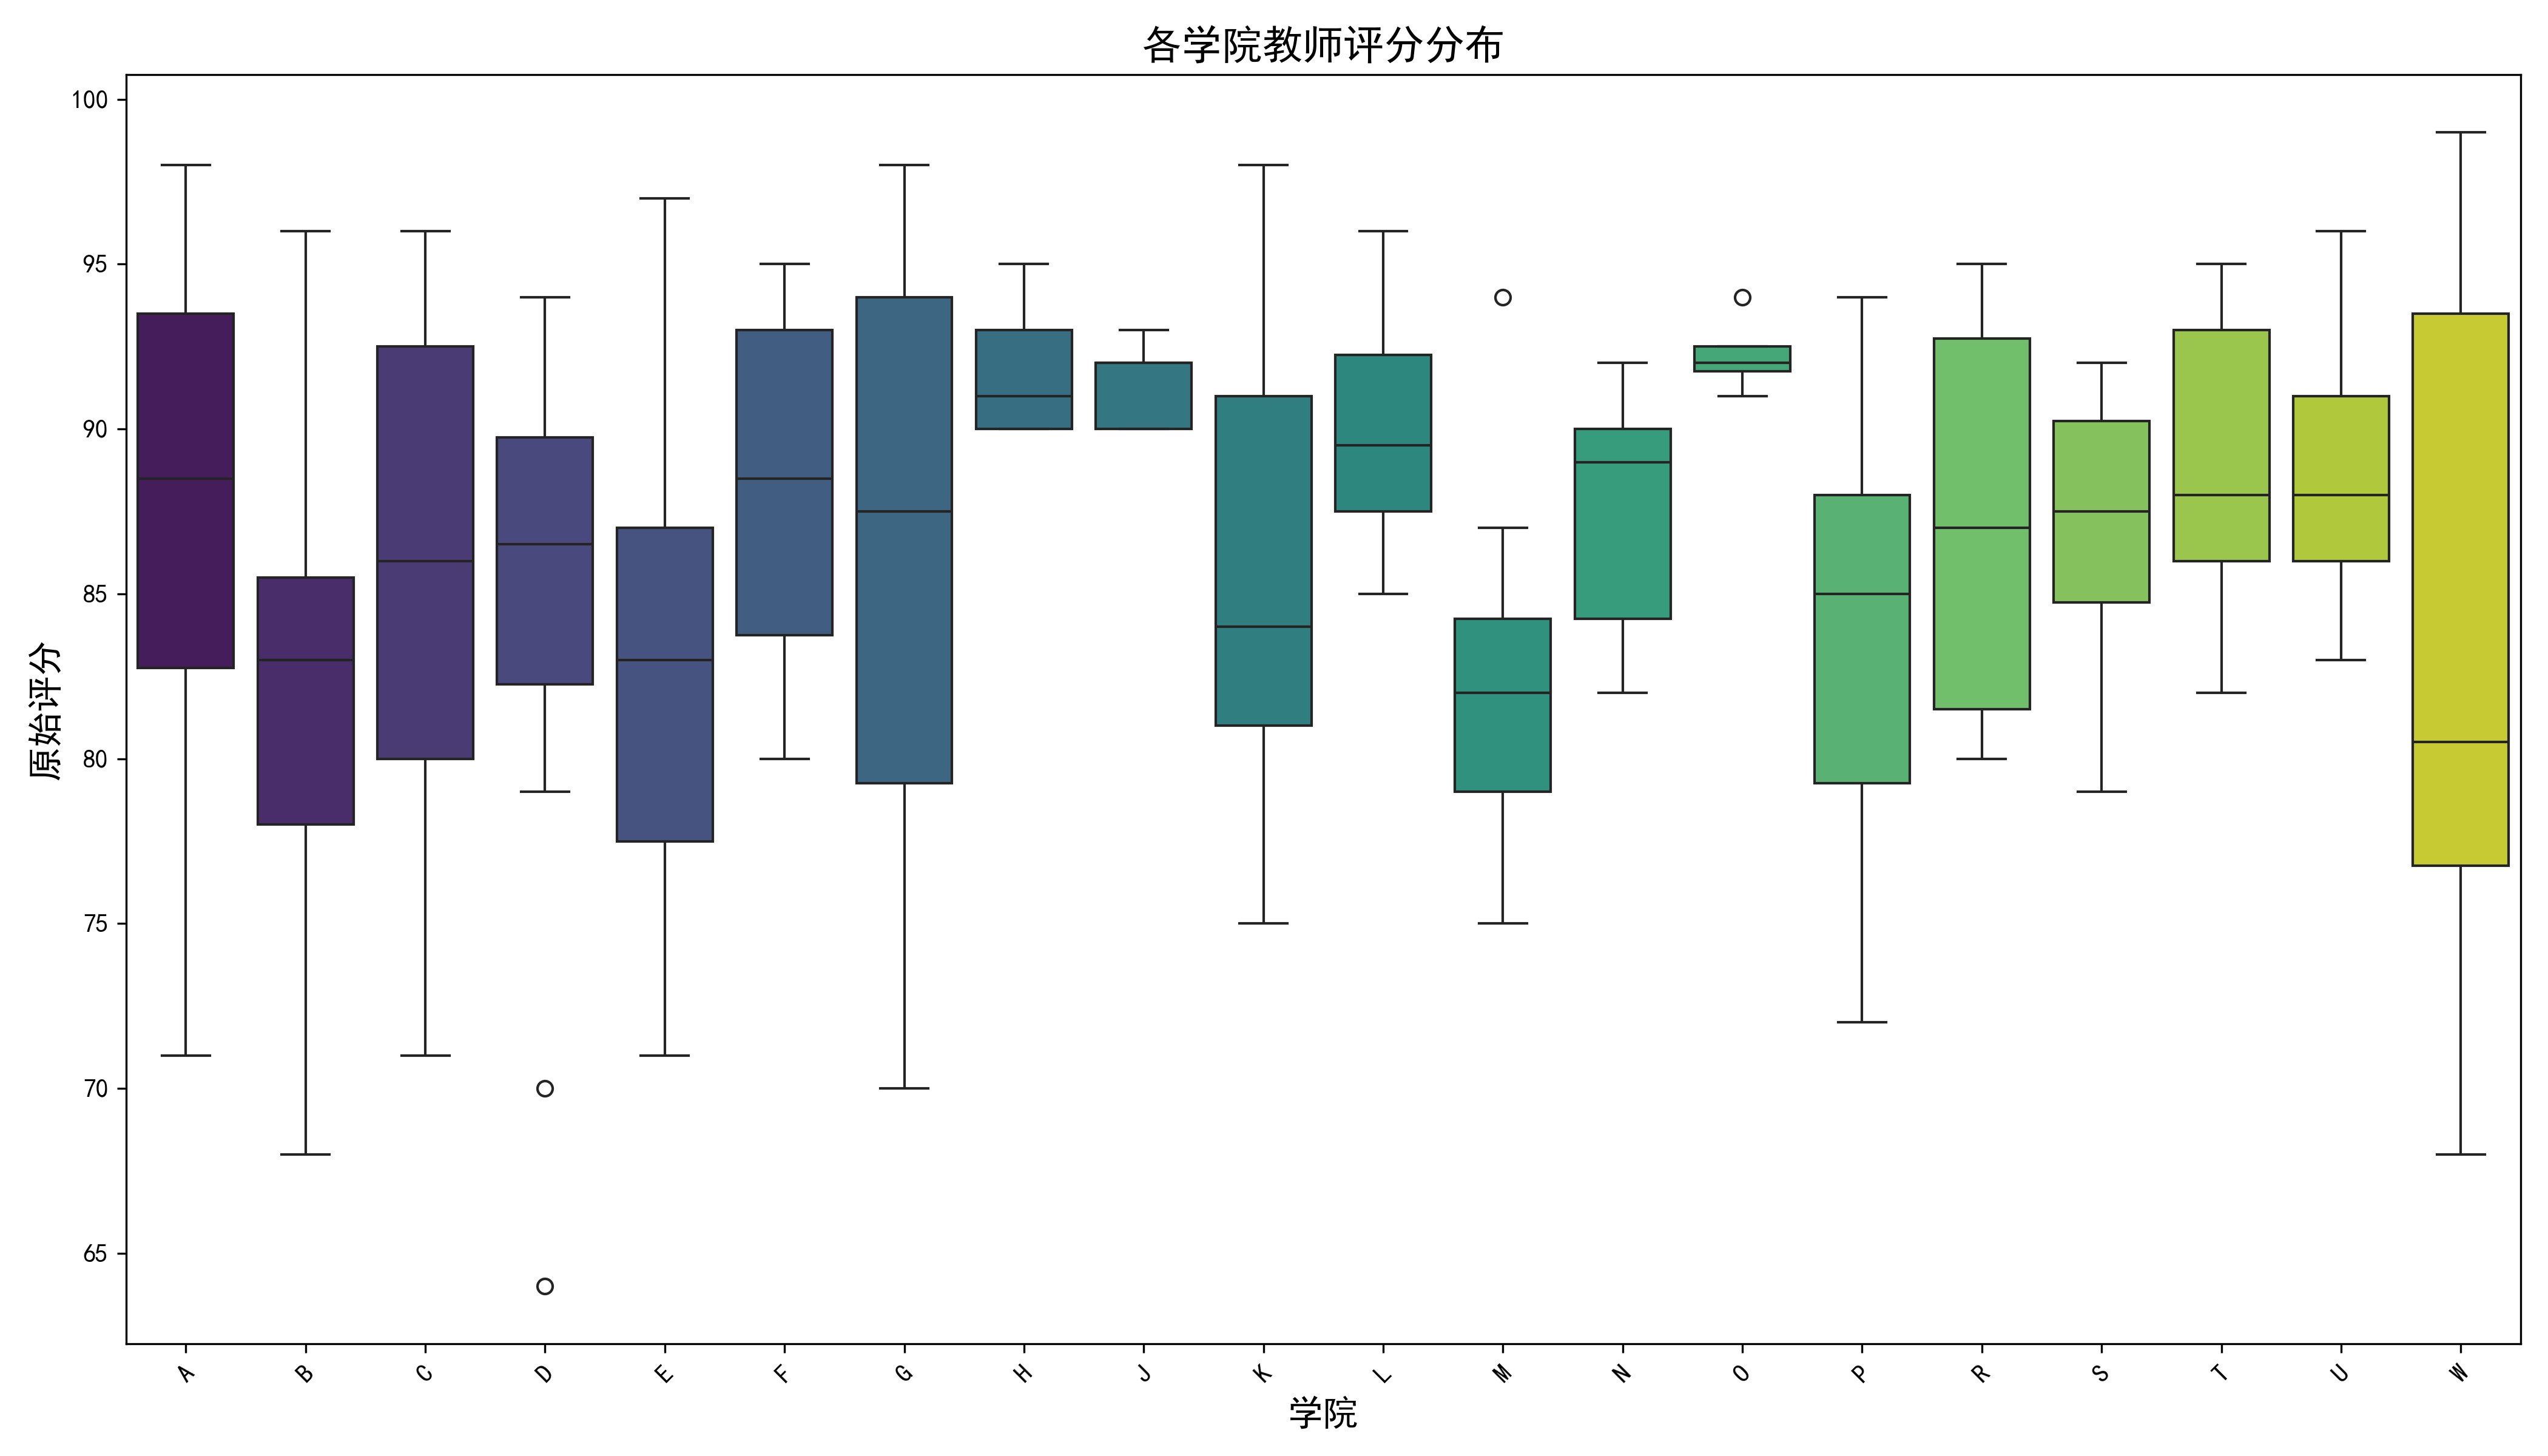
\includegraphics[width=0.75\textwidth]{figures/EDA/college_scores_boxplot.png}
% \caption{各学院原始分数分布箱线图}
% \label{fig:college_scores_boxplot}
% \end{figure}



\subsection{模型求解}


% \begin{figure}[H]
% \centering
% 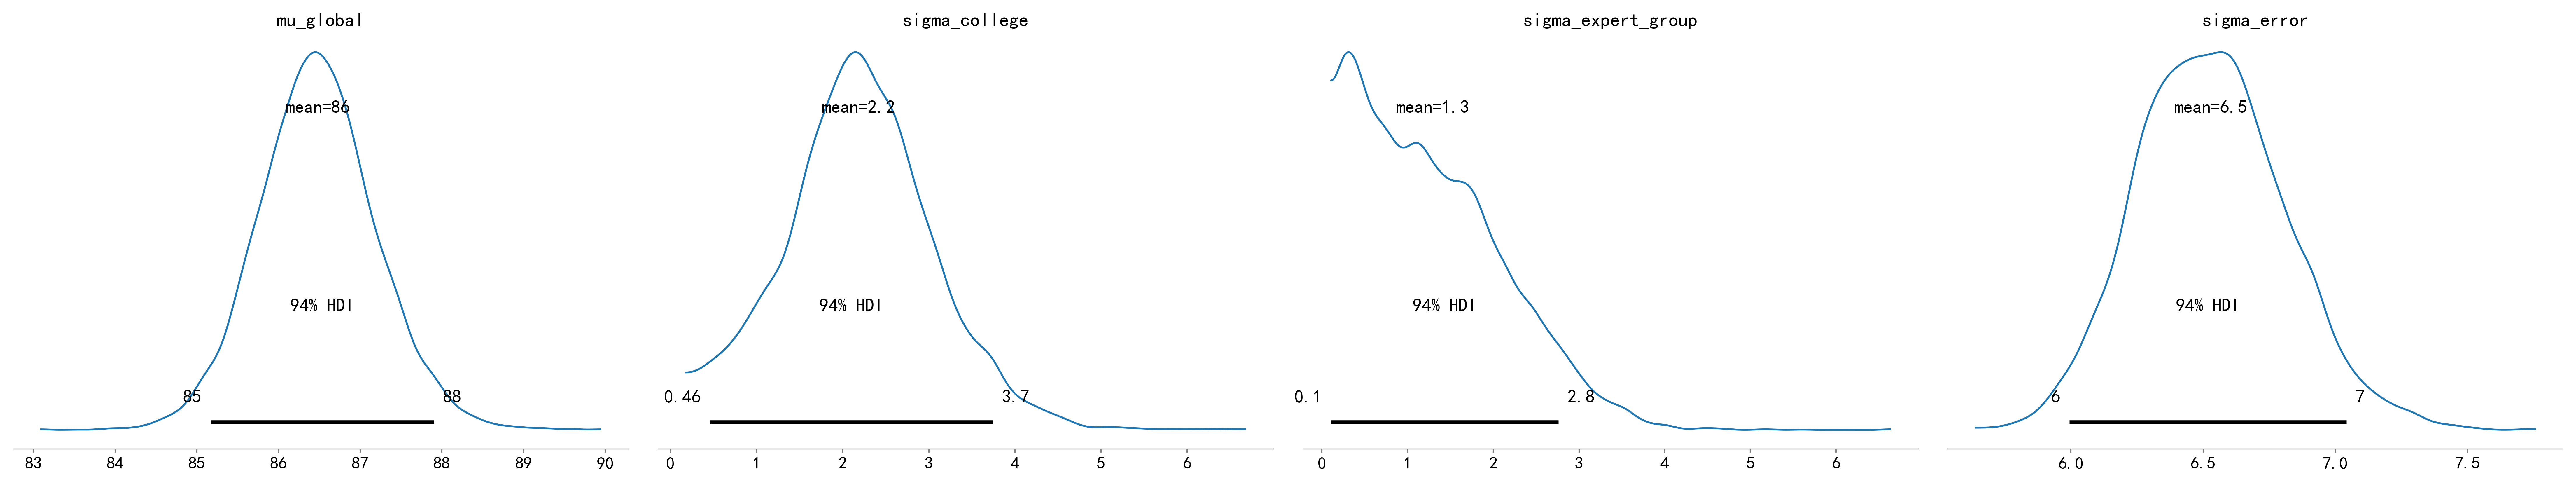
\includegraphics[width=1\textwidth]{figures/Diagnostics/posterior_plots.png}
% \caption{主要参数后验分布图}
% \label{fig:posterior_plots}
% \end{figure}

% \begin{figure}[H]
% \centering
% 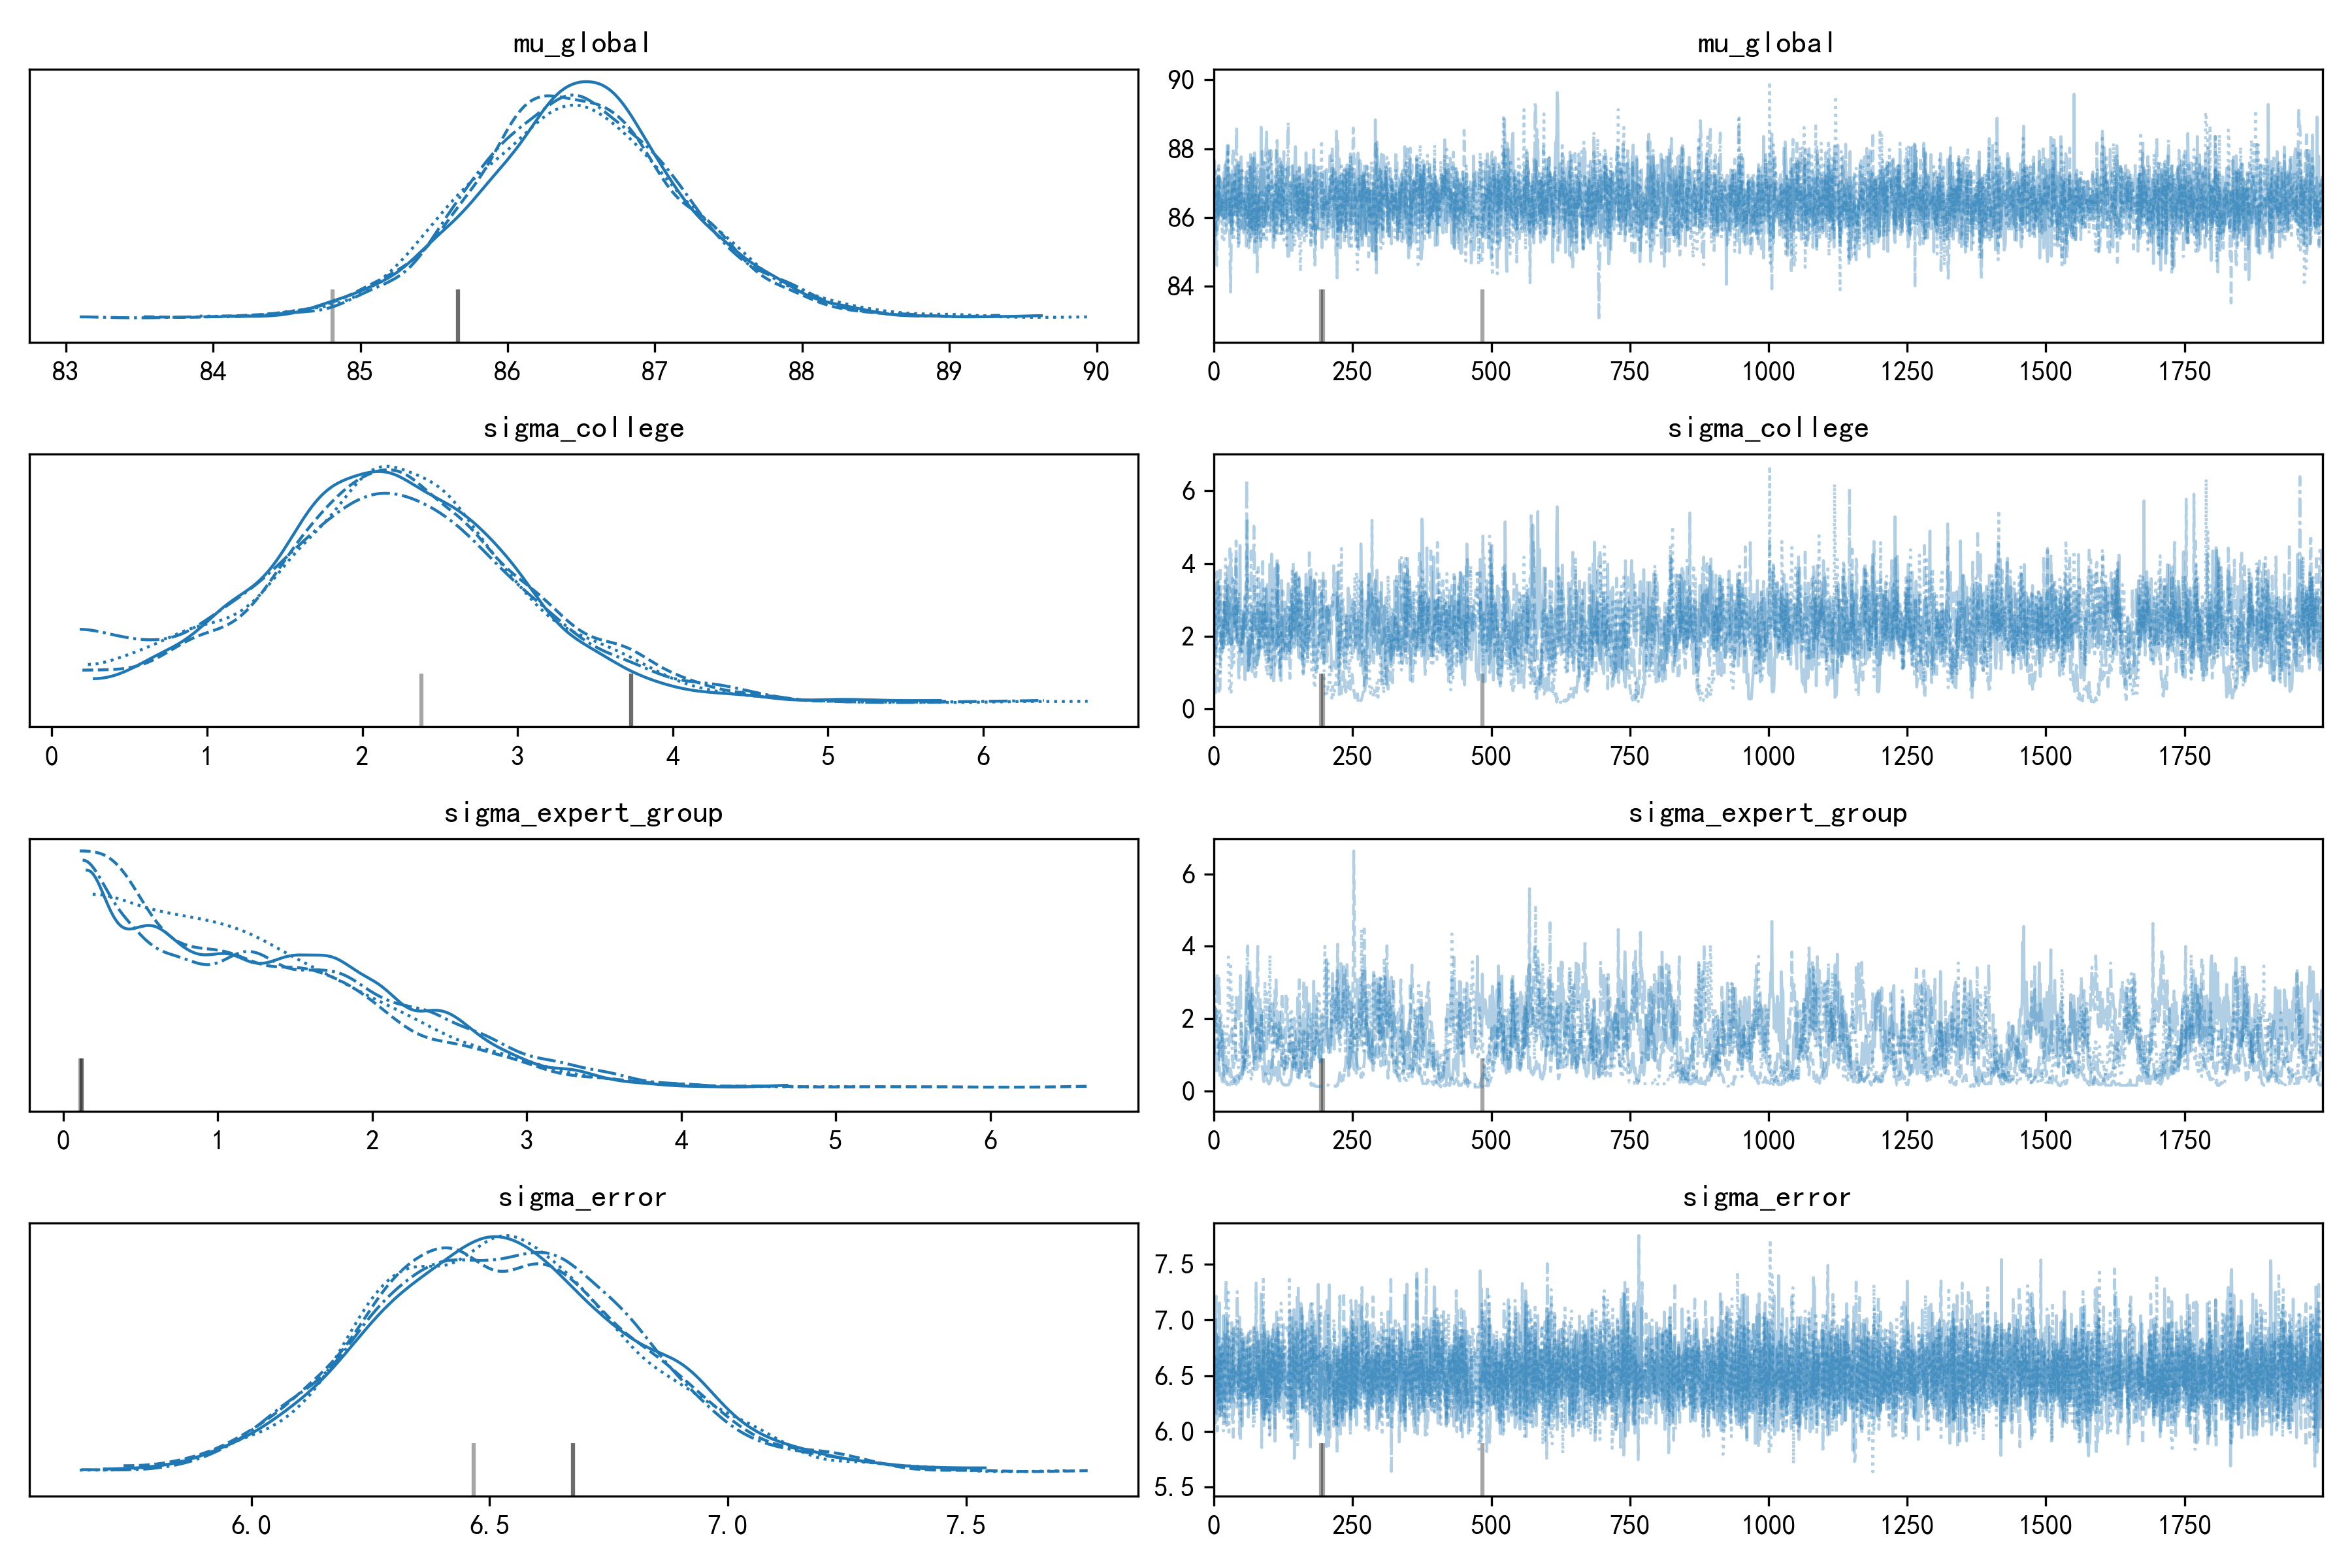
\includegraphics[width=1\textwidth]{figures/Diagnostics/trace_plots.png}
% \caption{MCMC采样traceplot诊断图}
% \label{fig:trace_plots}
% \end{figure}


% \begin{figure}[H]
% \centering
% 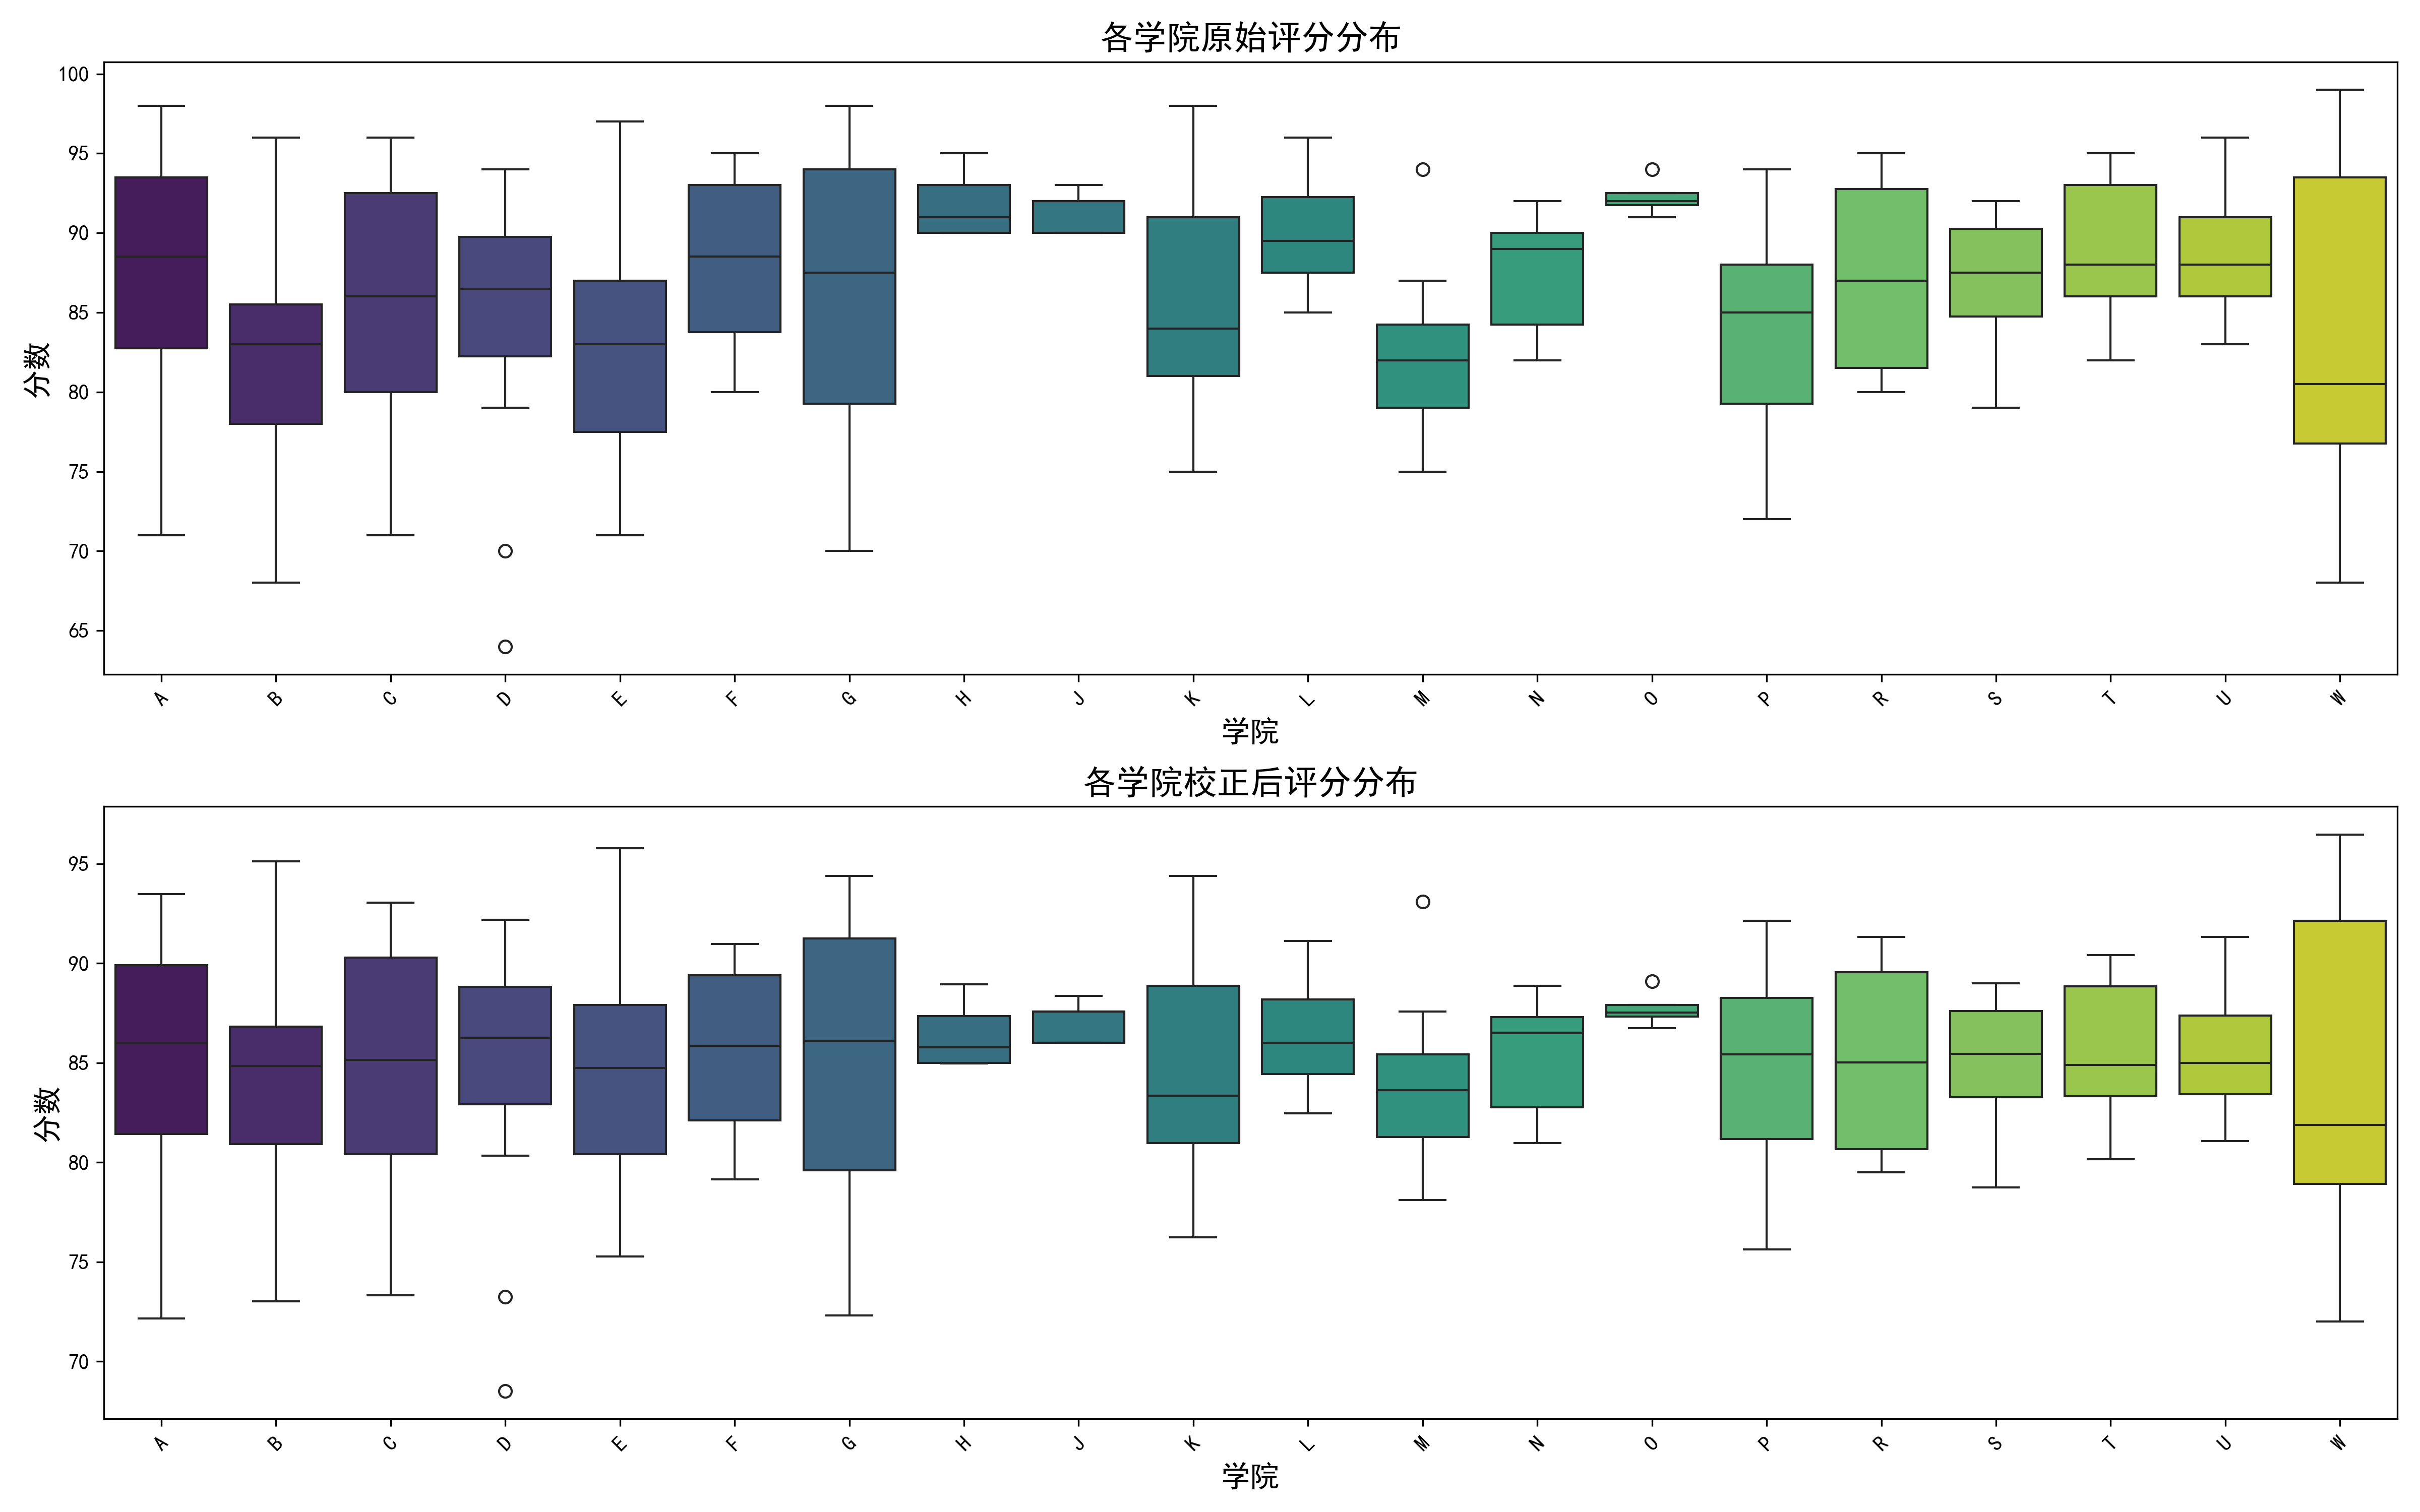
\includegraphics[width=1\textwidth]{figures/Results_Visualization/college_scores_comparison.png}
% \caption{校正前后各学院分数分布对比}
% \label{fig:college_scores_comparison}
% \end{figure}

% 教师排名和分数分布的变化见图6和图7,可以看出模型提升了整体的公平性。

% \begin{figure}[H]
% \centering
% 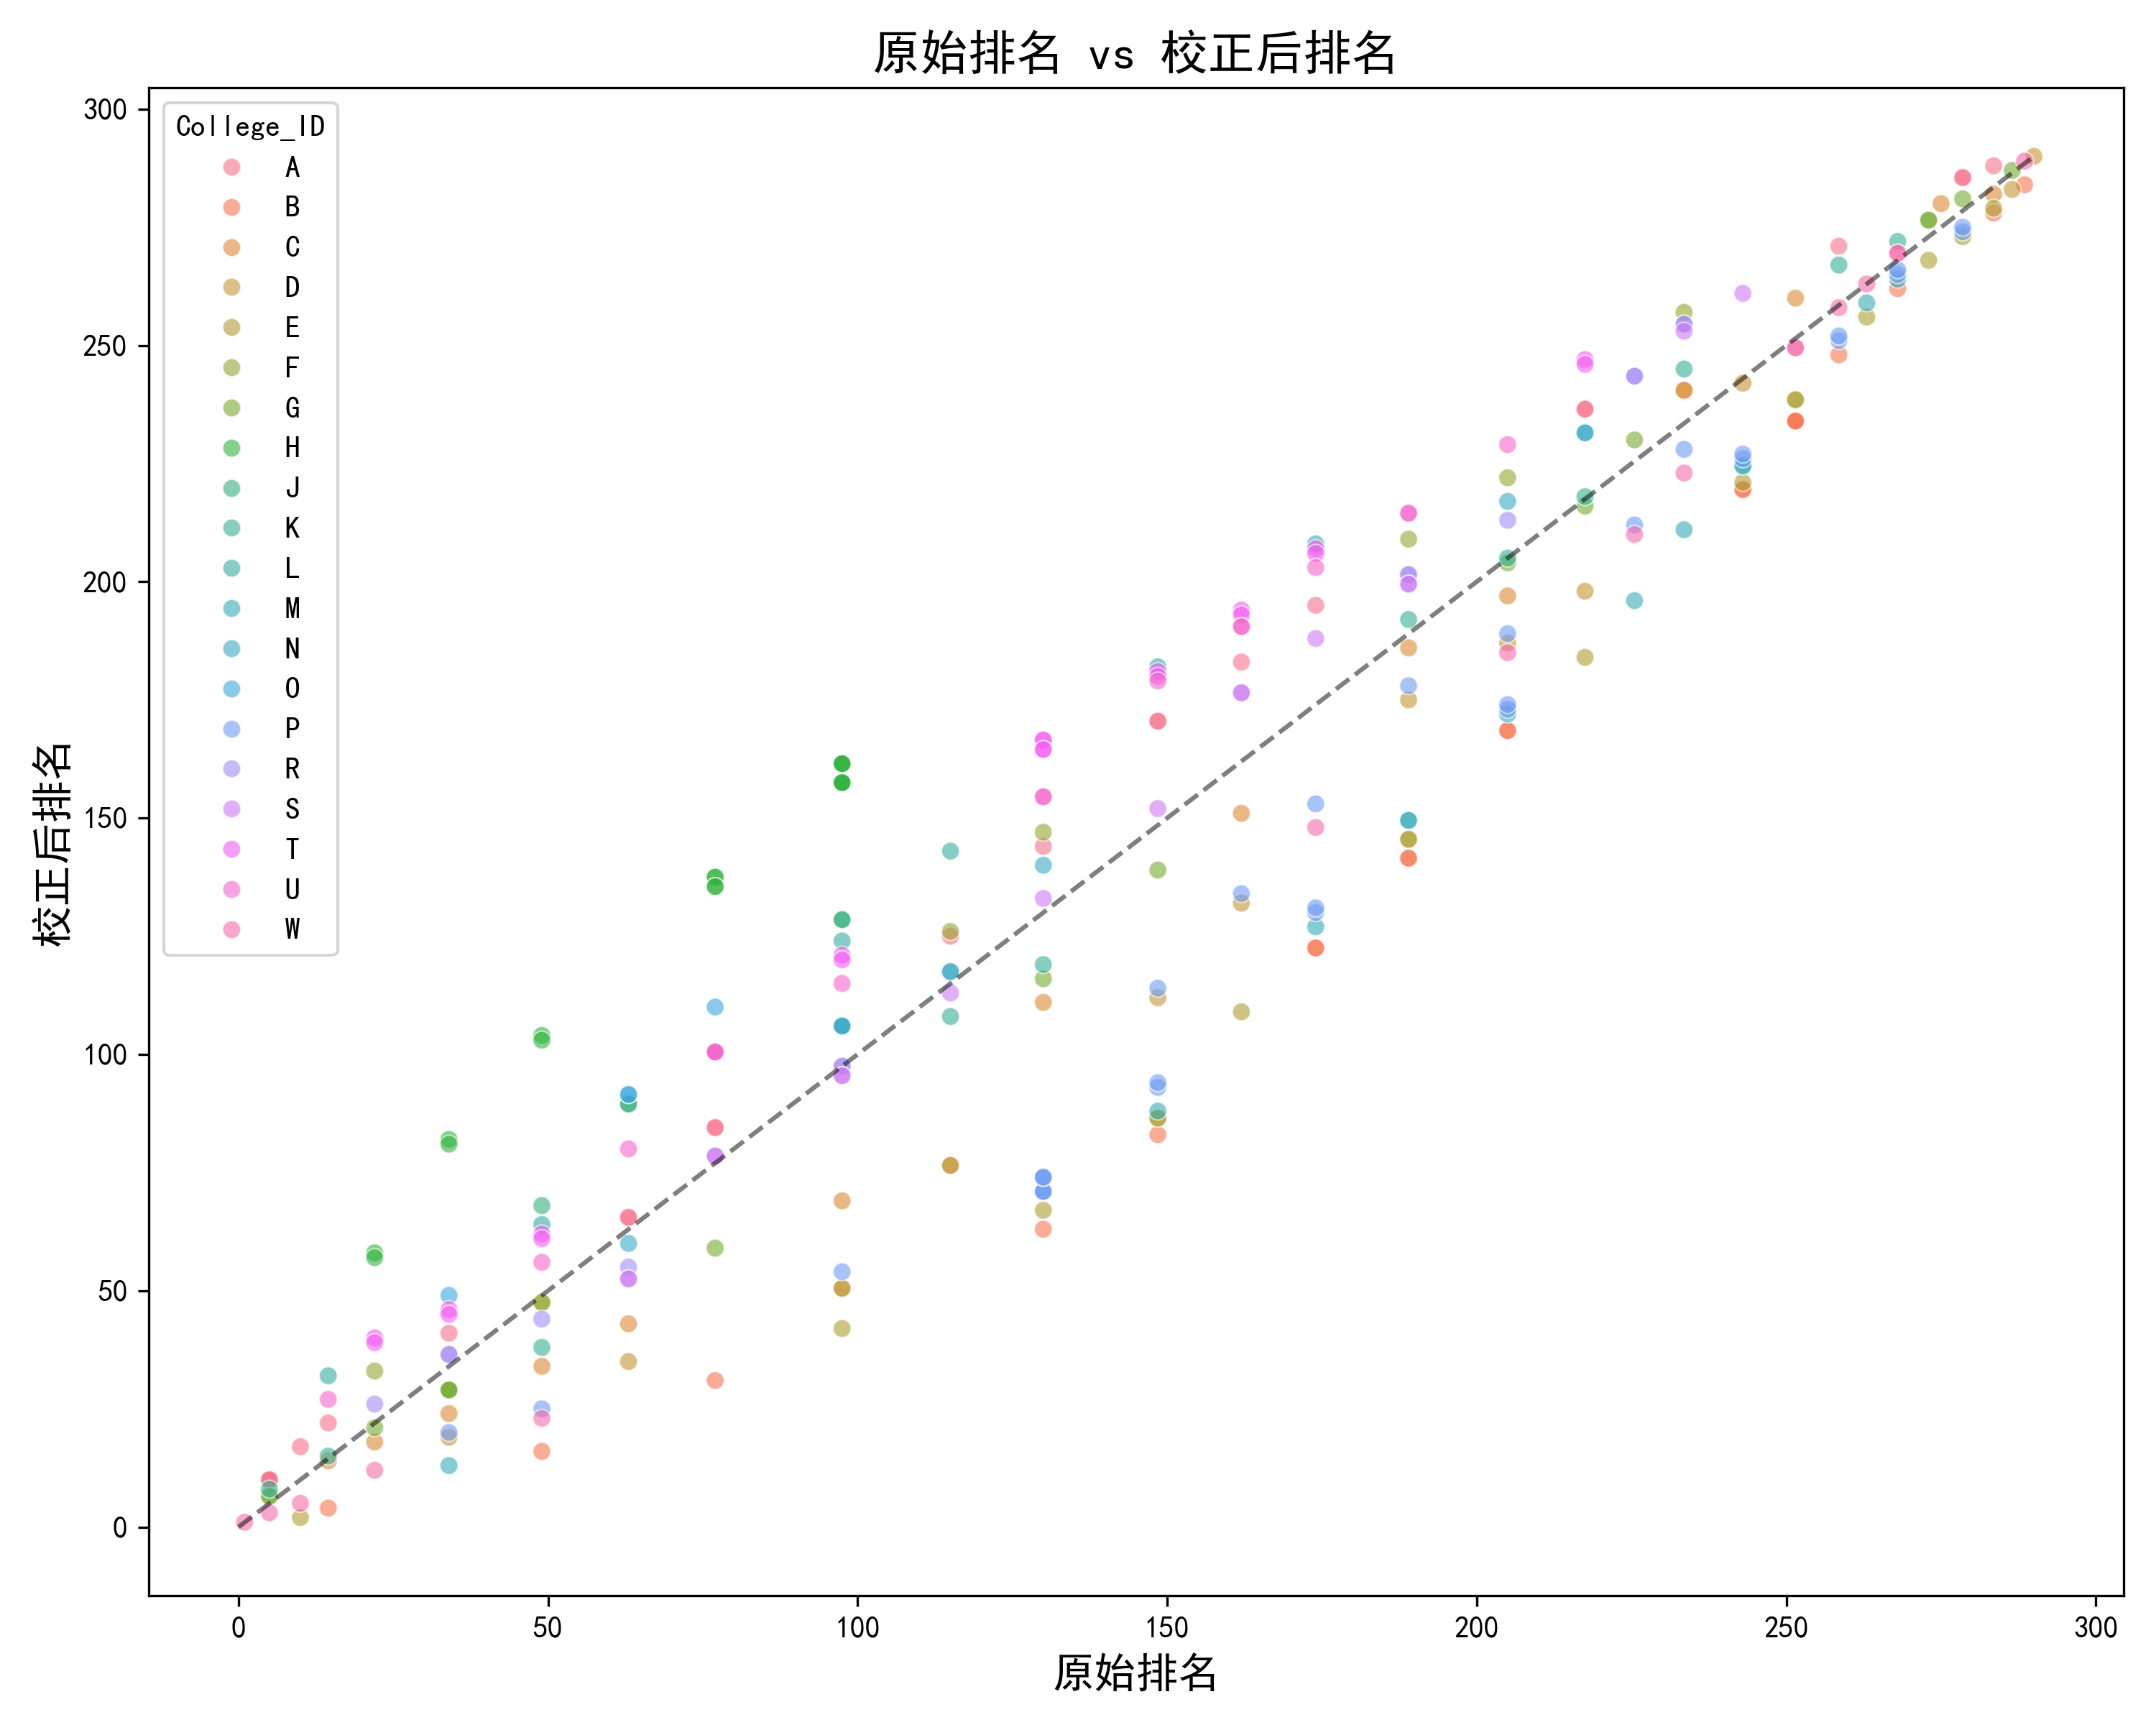
\includegraphics[width=1\textwidth]{figures/Results_Visualization/rank_comparison_scatter.png}
% \caption{校正前后教师排名变化散点图}
% \label{fig:rank_comparison_scatter}
% \end{figure}

% \begin{figure}[H]
% \centering
% 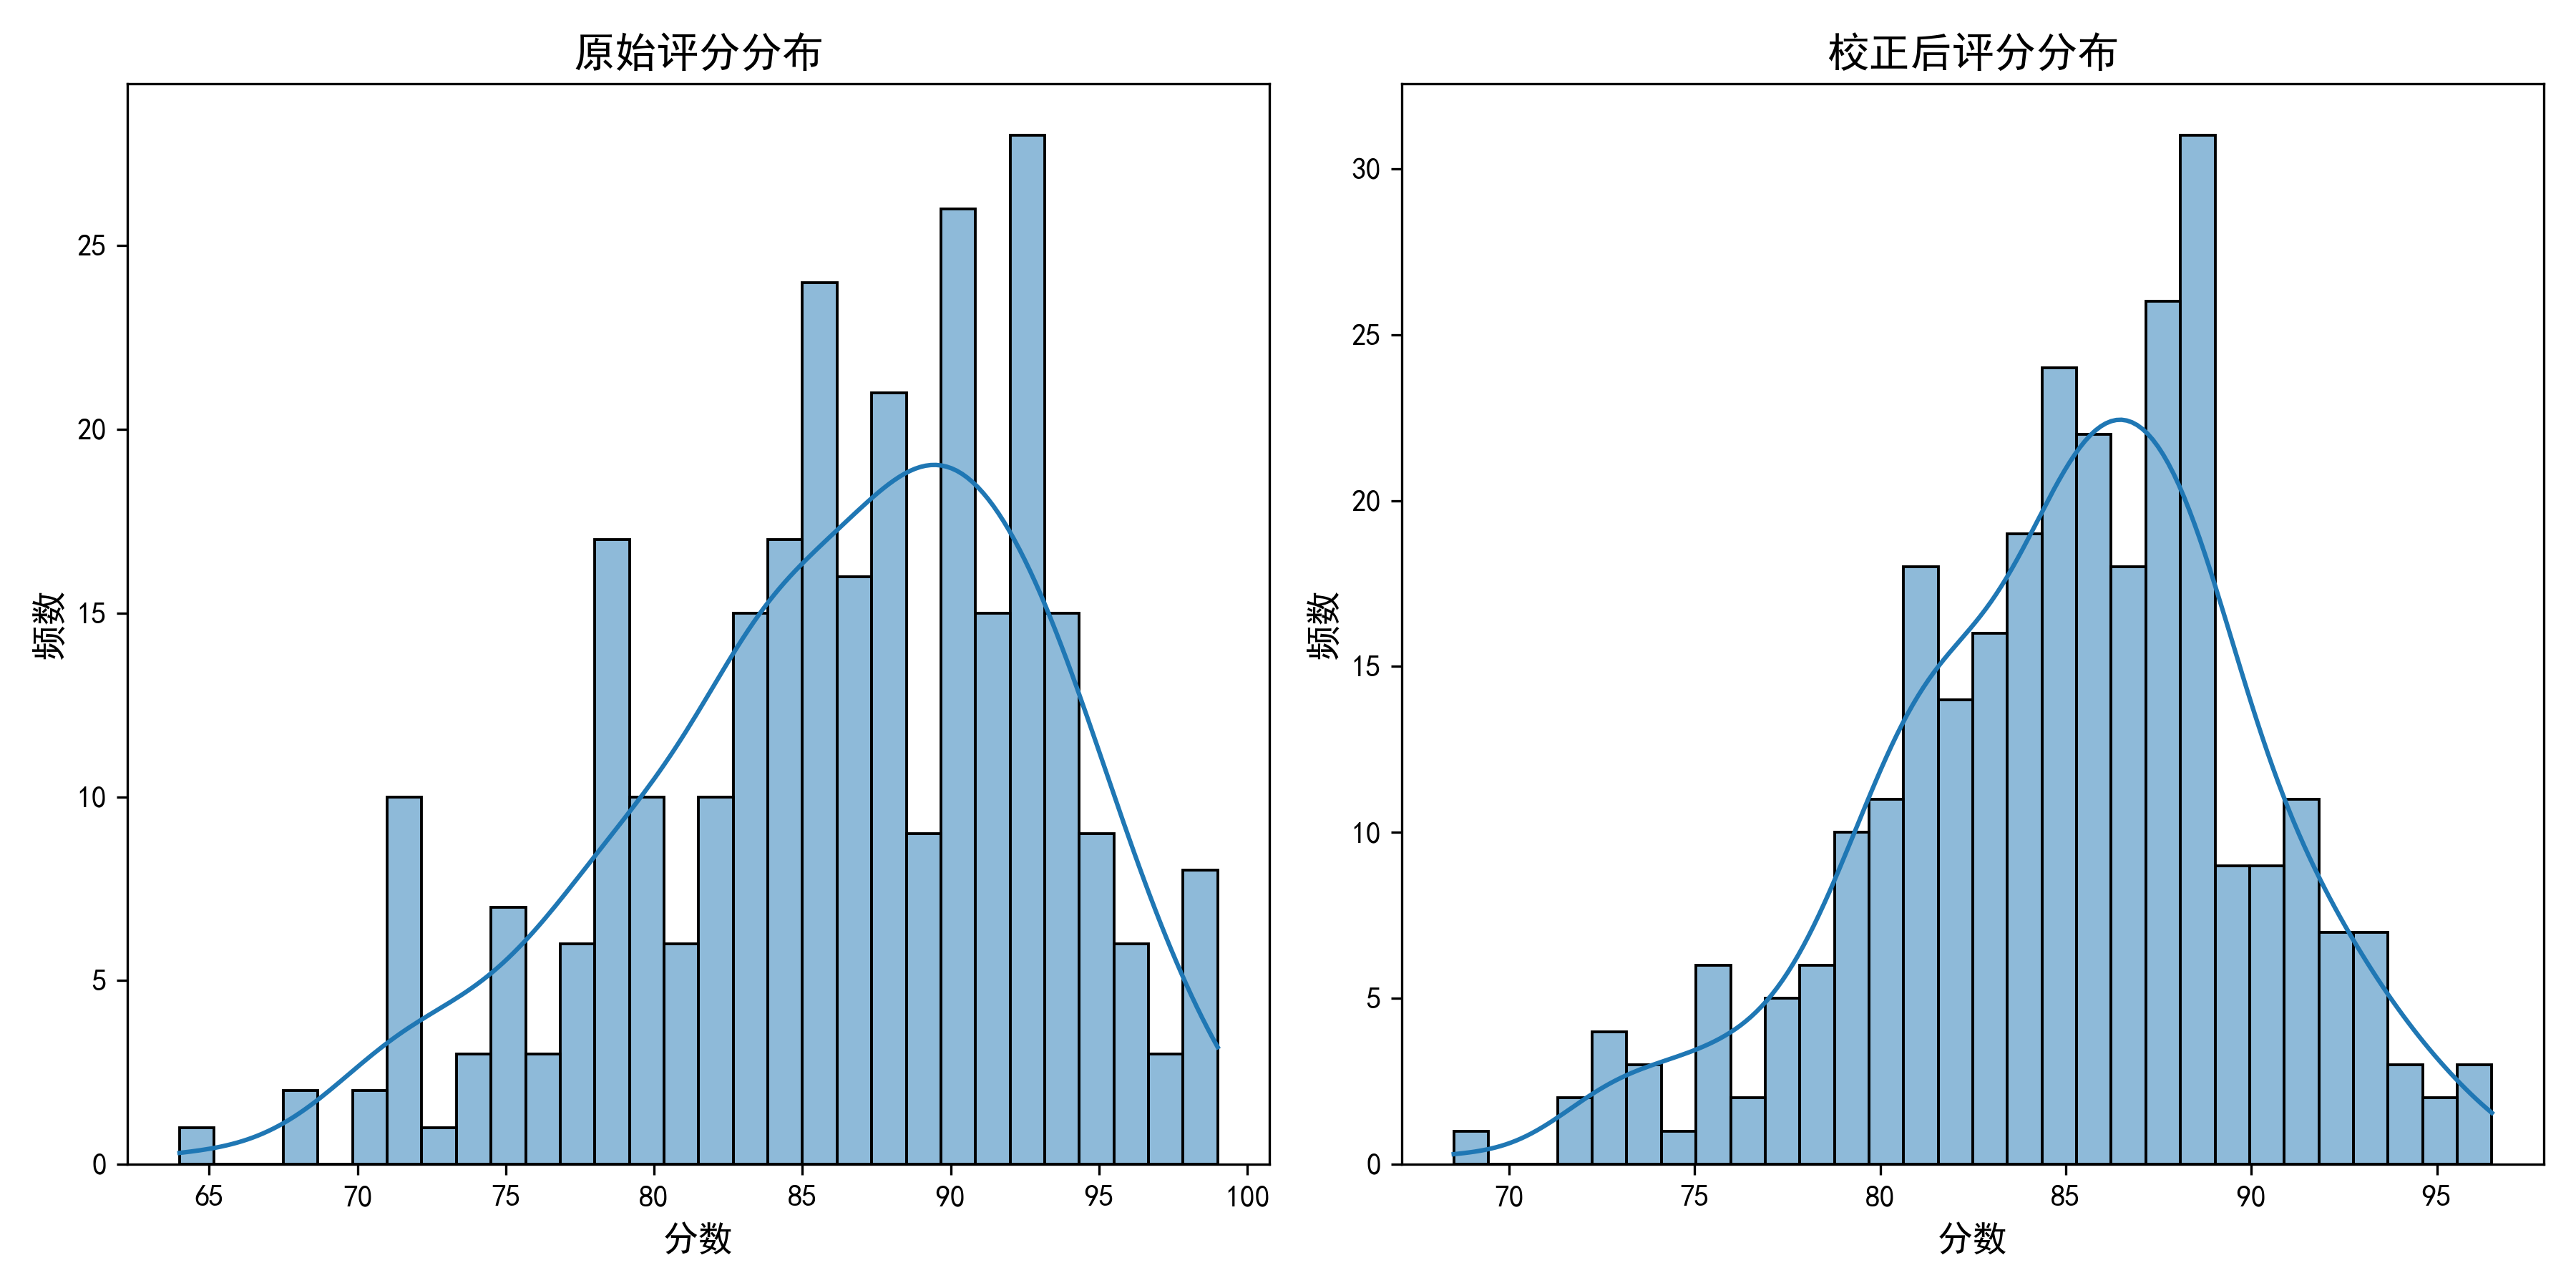
\includegraphics[width=1\textwidth]{figures/Results_Visualization/score_distributions_comparison.png}
% \caption{分数分布直方图对比,校正后分布更接近正态}
% \label{fig:score_distributions_comparison}
% \end{figure}



% \section{问题二的模型的建立和求解}
% \subsection{模型建立}

% 引用\cref{fig:双图},引用\cref{fig:双图a},引用\cref{fig:双图b}。

% \begin{figure}[ht]
% \centering
% \subcaptionbox{双图a子标题\label{fig:双图a}}
% {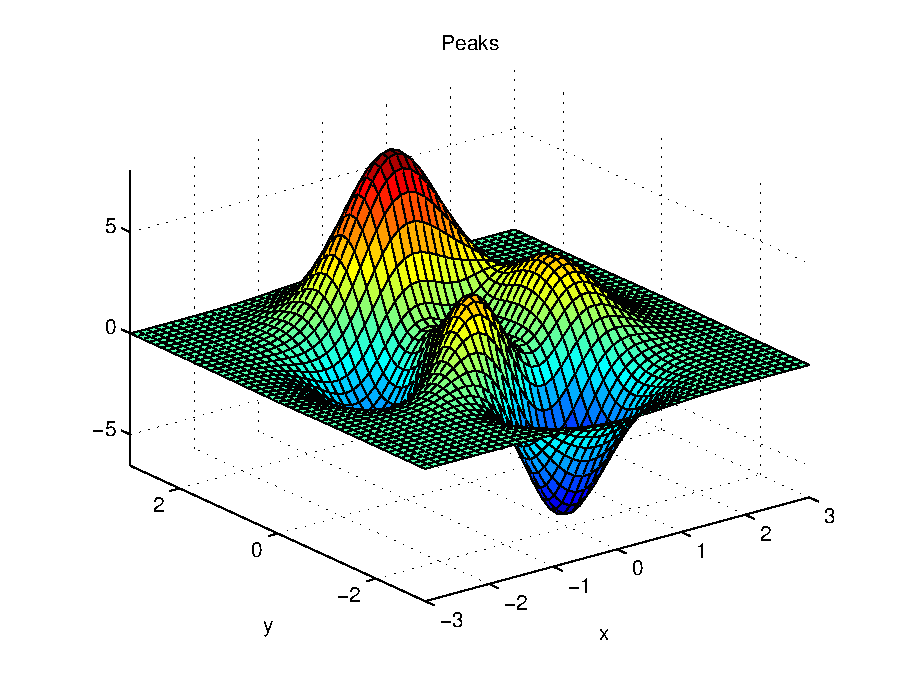
\includegraphics[width=.4\textwidth]{example.eps}}
% \subcaptionbox{双图b子标题\label{fig:双图b}}
% {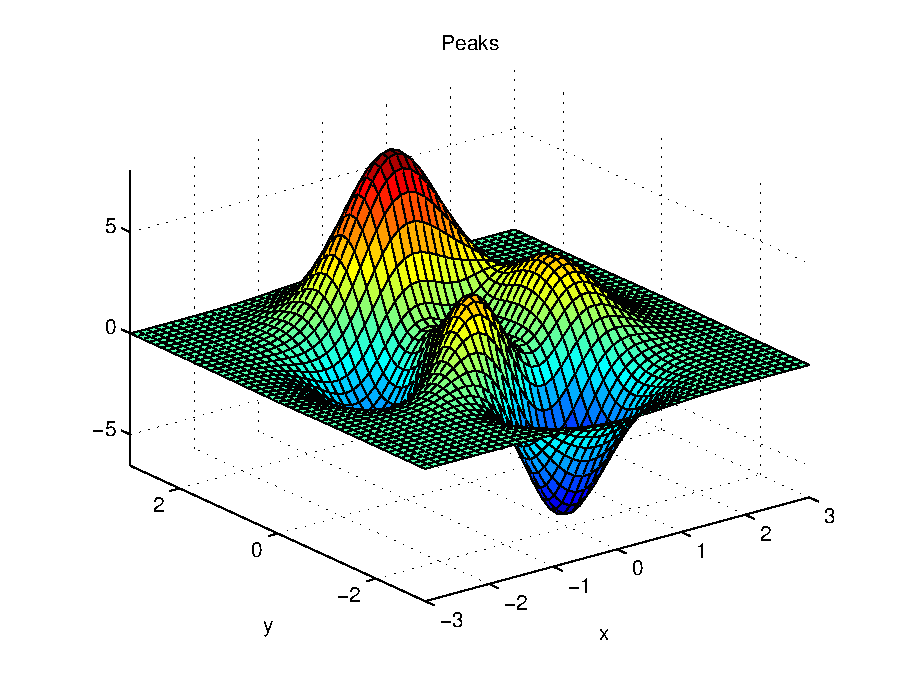
\includegraphics[width=.4\textwidth]{example.eps}}
% \caption{双图}\label{fig:双图}
% \end{figure} 

% \subsection{模型求解}

% \textbf{Step1:} 

% \textbf{Step2:} 

% \textbf{Step3:} 

% \subsection{求解结果}

% %%%%%%%%%%%%%%%%%%%%%%%%%%%%%%%%%%%%%%%%%%%%%%%%%%%%%%%%%%%%% 

% \section{问题三的模型的建立和求解}
% \subsection{模型建立}

% \subsection{模型求解}

% \textbf{Step1:} 

% \textbf{Step2:} 

% \textbf{Step3:} 

% \subsection{求解结果}

% %%%%%%%%%%%%%%%%%%%%%%%%%%%%%%%%%%%%%%%%%%%%%%%%%%%%%%%%%%%%% 

% \section{问题四的模型的建立和求解}
% \subsection{模型建立}

% \subsection{模型求解}

% \textbf{Step1:} 

% \textbf{Step2:} 

% \textbf{Step3:} 

% \subsection{求解结果}

% %%%%%%%%%%%%%%%%%%%%%%%%%%%%%%%%%%%%%%%%%%%%%%%%%%%%%%%%%%%%%

% \section{模型的分析与检验}

% \subsection{灵敏度分析}

% \subsection{误差分析}

% %%%%%%%%%%%%%%%%%%%%%%%%%%%%%%%%%%%%%%%%%%%%%%%%%%%%%%%%%%%%%

% \section{模型的评价}

% \subsection{模型的优点}
% \begin{itemize}[itemindent=2em]
% \item 优点1
% \item 优点2
% \item 优点3
% \end{itemize}

% \subsection{模型的缺点}
% \begin{itemize}[itemindent=2em]
% \item 缺点1
% \item 缺点2
% \end{itemize}

%%%%%%%%%%%%%%%%%%%%%%%%%%%%%%%%%%%%%%%%%%%%%%%%%%%%%%%%%%%%%
%% 参考文献
% \nocite{*}
% \bibliographystyle{gbt7714-numerical}  % 引用格式
% \bibliography{ref.bib}  % bib源


\begin{thebibliography}{99}


\end{thebibliography}

% 附录A之前插入参考文献
\begin{appendices}
% ...existing code...
\section{代码}
% \noindent 1:数据预处理
% \lstinputlisting[language=python]{code/excel_to_csv.py}
% 2:问题一模型
% \lstinputlisting[language=python]{code/problem1_solution.py}
% 3:问题二模型
% \lstinputlisting[language=python]{code/problem2_solution.py}

\end{appendices}
\end{document}



